\documentclass{article}

\setlength{\headsep}{0.75 in}
\setlength{\parindent}{0 in}
\setlength{\parskip}{0.1 in}

%=====================================================
% Add PACKAGES Here (You typically would not need to):
%=====================================================

\usepackage[margin=1in]{geometry}
\usepackage{amsmath,amsthm}
\usepackage{fancyhdr}
\usepackage{enumitem}
\usepackage{graphicx}
%=====================================================
% Ignore This Part (But Do NOT Delete It:)
%=====================================================

\theoremstyle{definition}
\newtheorem{problem}{Problem}
\newtheorem*{fun}{Fun with Algorithms}
\newtheorem*{challenge}{Challenge Yourself}
\def\fline{\rule{0.75\linewidth}{0.5pt}}
\newcommand{\finishline}{\vspace{-15pt}\begin{center}\fline\end{center}}
\newtheorem*{solution*}{Solution}
\newenvironment{solution}{\begin{solution*}}{{\finishline} \end{solution*}}
\newcommand{\grade}[1]{\hfill{\textbf{($\mathbf{#1}$ points)}}}
\newcommand{\thisdate}{\today}
\newcommand{\thissemester}{\textbf{Rutgers: Spring 2021}}
\newcommand{\thiscourse}{CS 440: Introduction to Artificial Intelligence} 
\newcommand{\thishomework}{Number} 
\newcommand{\thisname}{Name} 

\newcommand{\thisheading}{
   \noindent
   \begin{center}
   \framebox{
      \vbox{\vspace{2mm}
    \hbox to 6.28in { \textbf{\thiscourse \hfill \thissemester} }
       \vspace{4mm}
       \hbox to 6.28in { {\Large \hfill Project \#\thishomework \hfill} }
       \vspace{2mm}
         \hbox to 6.28in { { \hfill \thisdate \hfill} }
       \vspace{2mm}
       \hbox to 6.28in { \emph{Names: \thisname \hfill }}
      \vspace{2mm}}
      }
   \end{center}
   \bigskip
}

%=====================================================
% Some useful MACROS (you can define your own in the same exact way also)
%=====================================================


\newcommand{\ceil}[1]{{\left\lceil{#1}\right\rceil}}
\newcommand{\floor}[1]{{\left\lfloor{#1}\right\rfloor}}
\newcommand{\prob}[1]{\Pr\paren{#1}}
\newcommand{\expect}[1]{\Exp\bracket{#1}}
\newcommand{\var}[1]{\textnormal{Var}\bracket{#1}}
\newcommand{\set}[1]{\ensuremath{\left\{ #1 \right\}}}
\newcommand{\poly}{\mbox{\rm poly}}


%=====================================================
% Fill Out This Part With Your Own Information:
%=====================================================


\renewcommand{\thishomework}{1: This Maze is on \emph{Fire}} %Homework number
\renewcommand{\thisname}{Aamna Farooq, Nada Elshamaa, and Asma Makhdoom} % Your name
 \graphicspath{ {./images/} }

\begin{document}

\thisheading



\begin{problem}
	Write an algorithm for generating a maze with a given dimension and obstacle density p.
	 
\end{problem}
\begin{solution}
	The solution to problem one goes here. 
		
%=====================================================
% LaTeX Tip: The figure environment is used for displaying the figure. Inside that, we use \includegraphics for adding a different file for each of the figure.
% What you need to do is to create your figure using any tool you like (including drawing it by hand and scanning it), turn it into a pdf, name it "tree[X].pdf" 
% where you replace [X] by A,B,C, or D depending on which part you are solving (i.e., use treeA.pdf, treeB.pdf,...). Finally, copy the file in the same directory
% as this template and you should see that getting compiled into your solution. You can change the width=0.5\textwidth command to fix the size of the figure
% in the final PDF. Finally, if the figure appears in the next page, do not worry about it as they will still have the proper caption. 
%=====================================================		
\end{solution}
\smallskip

\begin{problem}
	Write a $DFS$ algorithm that takes a maze and two locations within it, and determines whether one is reachable from the other. Why is $DFS$ a better choice than $BFS$ here? For as large a dimension as your system can handle, generate a plot of 'obstacle density p' vs 'probability that S can be reached from G'
	
\end{problem}

\smallskip

\begin{solution}
	Solution to problem two goes here. 
\end{solution}


\smallskip


\begin{problem}
	Write $BFS$ and $A*$ algorithms (using the euclidean distance metric) that take a maze and determine the shortest path from $S$ to $G$ if one exists. For as large a dimension as your system can handle, generate a plot of the average $'number$ $of$ $nodes$ $explored$ $by$ $BFS$ - $number$ $of$ $nodes$ $explored$ $by$ $A*$' vs $'obstacle$ $density$ $p'$. If there is no path from $S$ to $G$, what should this difference be? 
	
\end{problem}

\smallskip

\begin{solution}
    If there was no path from S to G then there would be no difference between the number of nodes explored. This is because A* and BFS each would try to exhaust every possible option and would therefore have the same number of nodes explored.
    
	\begin{figure}[h]
	\centering
	\IfFileExists{images/dim100,50avg,step01.png}{\includegraphics[width=0.7\textwidth]{images/dim100,50avg,step01.png}}{No Figure Yet}
% 	\includegraphics[width=12cm]{dim100,50avg,step01}
	\caption{Plot using a dimension of 1000, average of 50, 0<p<1 with step = 0.01}
	\end{figure}
	
\end{solution}

\smallskip

\begin{problem}
	What's the largest dimension you can solve using $DFS$ at p = 0.3 in $less$ than a minute? What's the largest dimension you can solve using $BFS$ at p = 0.3 in $less$ than a minute? What's the largest dimension you can solve using $A*$ at p = 0:3 in $less$ than a minute?  
\end{problem}

\smallskip

\begin{solution}
	Solution to problem four goes here. 
\end{solution}

\smallskip

\begin{problem}
	Describe your improved Strategy 3. How does it account for the unknown future?
\end{problem}

\smallskip

\begin{solution}
	Solution to problem four goes here. 
\end{solution}

\smallskip

\begin{problem}
	Plot, for Strategy 1, 2, and 3, a graph of `average strategy success rate' vs `flammability q' at p = 0.3. Where do the different strategies perform the same? Where do they perform differently? Why?
\end{problem}

\smallskip

\begin{solution}
    Strategy 1:
	\begin{figure}[h]
    \centerline{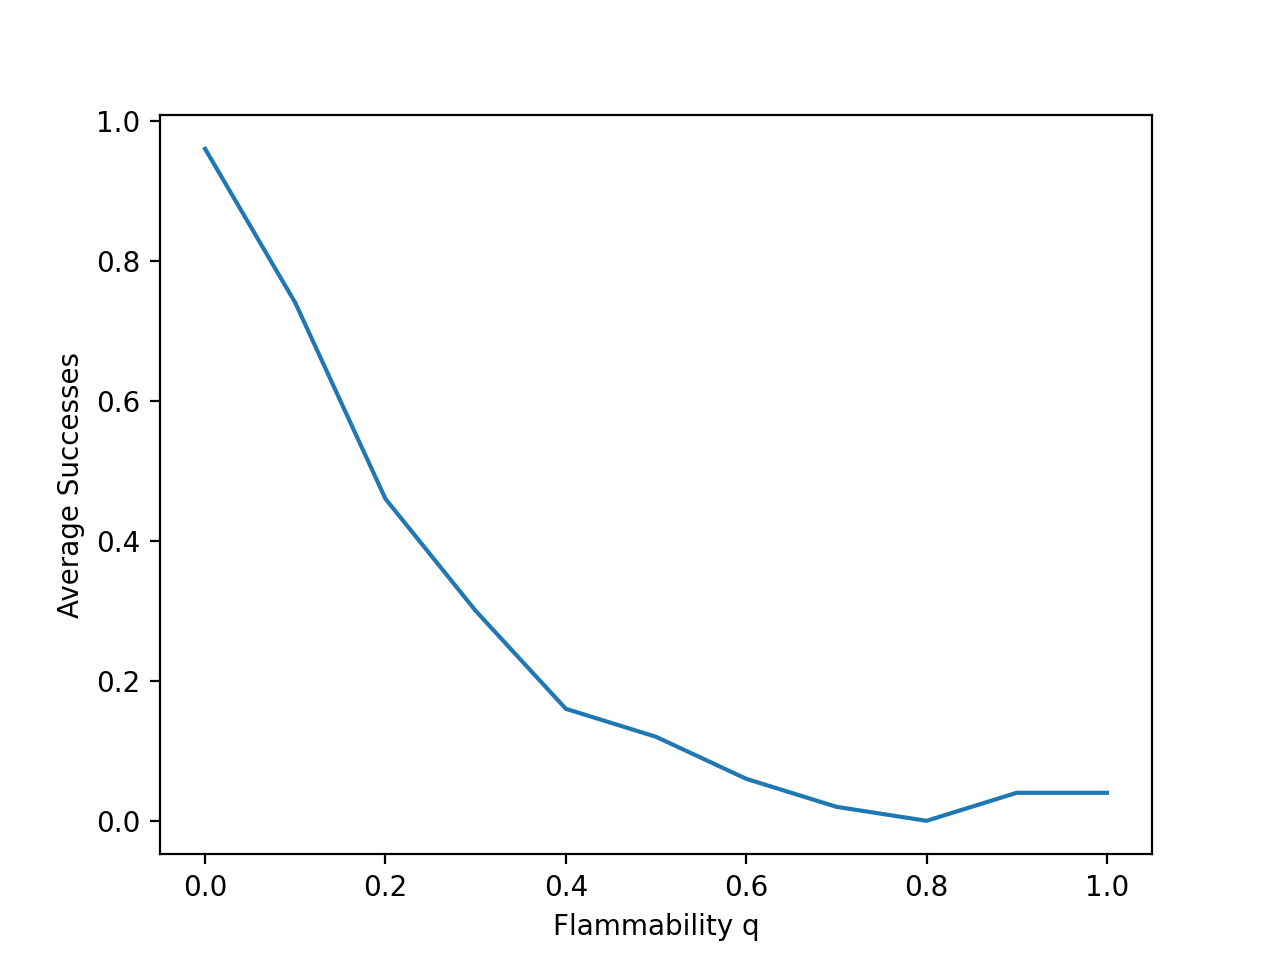
\includegraphics{P6ST1.png}}
    \caption{Strategy 1, Using a dimension of 100, average of 50, p=0.3, q with step of 0.1.}
    \label{fig}
    \end{figure}
 
    
    Strategy 2: 
    \begin{figure}[h]
    \centerline{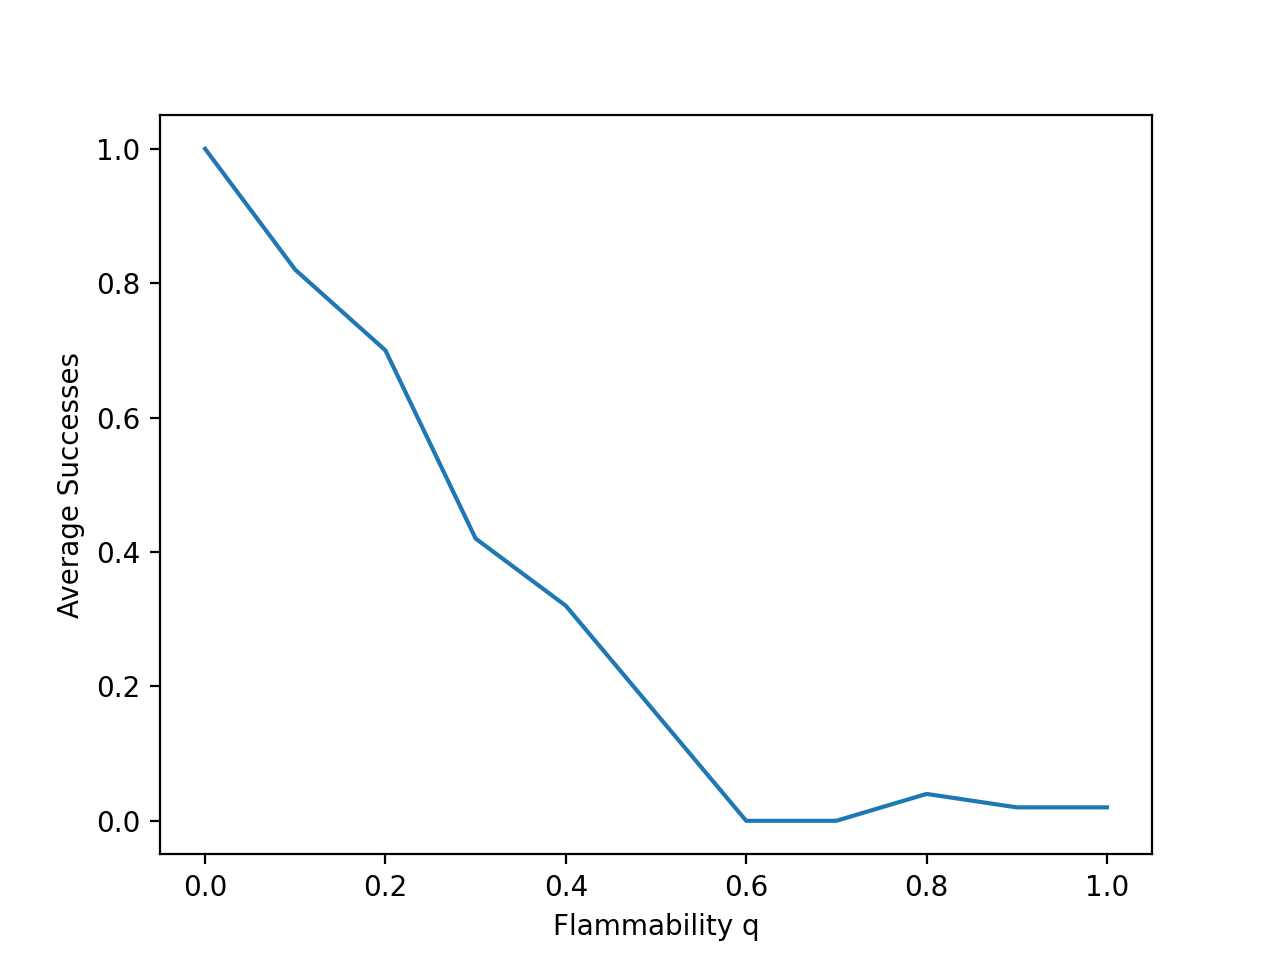
\includegraphics{P6ST2.png}}
    \caption{Strategy 2, Using a dimension of 100, average of 50, p=0.3, q with step of 0.1.}
    \label{fig}
    \end{figure}
    
    
    Strategy 3: 
    \begin{figure}[h]
    \centerline{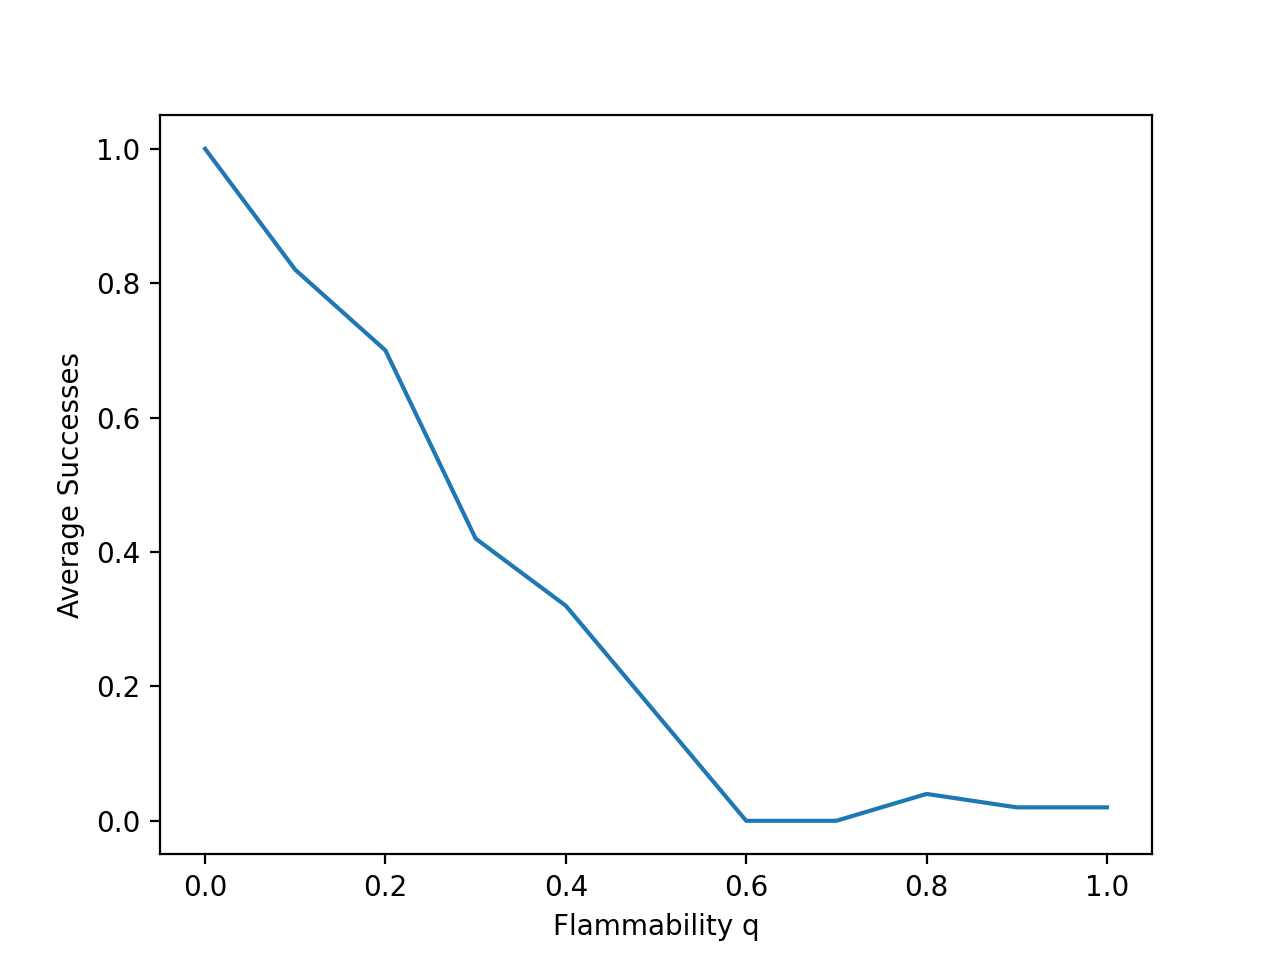
\includegraphics{P6ST2.png}}
    \caption{Strategy 3, Using a dimension of 100, average of 50, p=0.3, q with step of 0.1.}
    \label{fig}
    \end{figure}
\end{solution}

\smallskip

\begin{problem}
	If you had unlimited computational resources at your disposal, how could you improve on Strategy 3?
\end{problem}

\smallskip

\begin{solution}
	Solution to problem four goes here. 
\end{solution}

\smallskip

\begin{problem}
	If you could only take ten seconds between moves (rather than doing as much computation as you like), how would that change your strategy? Describe such a potential Strategy 4.
\end{problem}

\smallskip

\begin{solution}
	Solution to problem four goes here. 
\end{solution}

\smallskip

\end{document}